\chapter{Background and Literature Review}
\section{Understanding the Problem Domain}
%% Beam Injection:
%% TO DO
\paragraph{ }The purpose of the \ac{LHC} at \acs{CERN} is to accelerate and collide two proton beams \cite{Valentino2017}. In order to fill the \acs{LHC} with a beam of the required intensity, twelve injections consisting of a number of electron bunches of around 1 \acs{MJ} of stored energy each are required \cite{Drosdal2011}. This is a challenging task given the high energy of the beam, the very small apertures and the delivery precision's tight tolerances. Thus, multiple sensors are installed around the \acs{CERN} particle accelerator complex \cite{Lefevre2008} which gather readings and data that can be used to check the quality of the injected beam. 

%%The Particular area of interest to this study:
\paragraph{ }  For this particular study, data generated from the sensors around the injection from the \acs{SPS} to the \acs{LHC} will be of particular interest. This data is stored using \acs{CERN}'s \ac{LS} \cite{Roderick2013}. While many studies have been made using this logged data and lots of statistical tests have been done with regards to injection quality checks for the \acs{LHC} (such as \cite{Drosdal2011} and \cite{Kain2010}), no literature was uncovered where researchers used unsupervised machine learning methods to analyse this data. Figure \ref{fig::SPStoLHCInjection} highlights the particular area of interest of this study.

\begin{figure}[t]
	\centering
	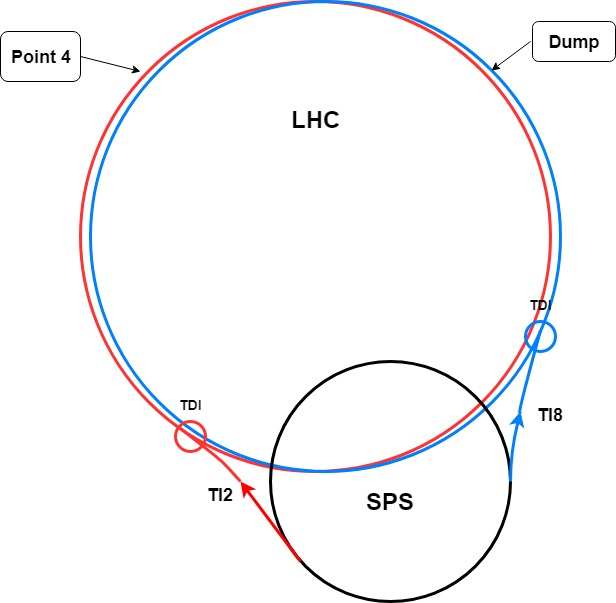
\includegraphics[width=0.4\textwidth]{CERNComplex}
	\caption[The CERN Particle Accelerator Complex]{Diagram of the particular area of interest of the CERN Particle Accelerator Complex for this study}
	\label{fig::SPStoLHCInjection}
\end{figure}

%% On the Current IQC software
\paragraph{ }The \ac{IQC} software currently installed has a set of hard-coded rules for detecting anomalies in the \acs{SPS}-\acs{LHC} injection \cite{Drosdal2011}, however there are documented cases in the past where situations occurred which were outside the originally foreseen rules and were therefore not caught as anomalies.
%% TO DO: Add some stuff from the Injection Quality PM Workshop

\section{The Instruments Used to Gather Data}
%Intro
\paragraph{ }Throughout this study, different data recorded as the beam leaves the \acs{SPS} and enters the \acs{LHC} was used as input parameters to the chosen anomaly detection algorithms. This data was recorded using different censors located in different parts of the injection life cycle. This section describes the different types of censors that were used to collect the data, highlighting the particular points which need to be considered when analysing the data.

%BLMs & TDI BLMs
\paragraph{ }The \ac{BLM} are some of the most safety critical modules of the \acs{LHC} because a loss of a very small fraction of this beam may damage parts of the machine or cause a quench in the superconducting magnets \cite{Holzer2006}. A high beam loss reading could also indicate over-injection. In fact, an injection of a high intensity beam into the LHC is only allowed if there is a low intensity bunch circulating the LHC in order to avoid settings errors \cite{Kain2010}. The \acs{BLM} module is the mostly used module in the current IQC checks \cite{Drosdal2011}. The \acs{BLM}s must be reliable; the probability of not detecting a dangerous loss was found to be $5\times10^{-6}$ per channel and they are only expected to generate 20 false dumps per year \cite{Holzer2006}. The \acs{BLM}s are extensively logged to a database for offline analysis \cite{Holzer2006}. 

\paragraph{ }For this particular study, the readings logged for the \ac{TDI} \acs{BLM}s and the \ac{TL} \acs{BLM}s in TI2 and TI8 will be used (refer to Figure \ref{fig::SPStoLHCInjection}). These readings come in 10 second windows around the injection of a bunch in \ac{Gy/s}.

%BPMs
\paragraph{ }The \ac{BPM} were installed as a system for fast monitoring of the beam's position with respect to it's orbit drift \cite{Schmidt2006}. The trajectory offsets recorded by the \acs{BLM}s in the transfer lines must be minimised in order to reduce losses \cite{Drosdal2011}. In fact, if the change in orbit substantially exceeds its provided boundary values then the beam should be dumped \cite{Schmidt2006} so as to not cause any damage to the equipment. Unlike the \acs{TDI} \acs{BLM}s, the \acs{BPM} system is independent to the collimator system. For this study, the readings from the transfer line \acs{BPM}s around TI2 and TI8 will be used (refer to Figure \ref{fig::SPStoLHCInjection}). Raw values for these readings are stored by the \acs{LS} in \ac{mm} and are logged every 1 - 5 seconds on average.

%Abort Gap
\paragraph{ }When filling the \acs{LHC}, it is necessary to keep an abort gap of at least 3$\mu s$ in order to accommodate for the \ac{MKD} rise time \cite{Meddahi2010}. As the \ac{LHC} is filling to nominal intensity, this gap will be populated with un-trapped particles and particles leaking out of their \ac{RF} buckets \cite{Meddahi2010}. The \ac{AGM} was hence specifically designed to measure this particle population in the abort gap \cite{Lefevre2010}. This monitor can be found in Point 4 (refer to Figure \ref{fig::SPStoLHCInjection}) in the LHC \cite{Lefevre2010}. The raw values extracted for this study are stored in number of particles and come in 10 second groups around the moment of injection.
 
%SPS and LHC Intensities
%TO DO 

%Number of Bunches
%TO DO


\section{Feature Scaling and Reduction Techniques}

%% Intro:
%% Curse of Dimensionality & Importance of Normalisation
\paragraph{ }Feature Scaling and Feature Reduction are two important pre-processing steps that should be considered when using machine learning in the data science process. Standard Scaling in particular will be used in this study as a pre-processing step to \ac{PCA}. This ensures that all the features have the properties of a standard normal distribution \cite{Scikitlearn}, which is especially important since \acs{PCA} involves finding the components that maximise the variance \cite{Shlens2014}. 

\paragraph{ }Data involving high dimensions can cause particular challenges for outlier detection algorithms as the contrast between different points diminishes as the number of dimensions increases \cite{Zimek2012}. This phenomenon is known as `The Curse of Dimensionality' and a technique to reduce the effect of this phenomenon is to use a dimension reduction technique and run the outlier detection algorithm on this new lower-dimensioned dataset. In this study, \acs{PCA} will be used as a dimension reduction technique.

%% PCA:
\paragraph{ }\acs{PCA} uses statistical and mathematical techniques to reduce the dimension of large data sets, thus allowing a large data set to be interpreted in less variables called principal components \cite{Richardson2009}. This technique works with the hope that the variance explained by an acceptably small number of principal components is large enough to explain the underlying structure of the dataset reasonably \cite{Shlens2014}. In fact, this non-parametric method has been used as a means of revealing the simplified structures underlying complex datasets with minimal effort. The fact that this technique is non-parametric gives it the advantage that each result is unique and only dependent on the provided data set since no parameter tweaking is required \cite{Shlens2014} however, this is also a weakness of this technique as there is no way of exploiting prior expert knowledge on the data set.

%% Recursive Feature Selection:
%% TO DO

%% Multilinear Discriminant Analysis (MDA)
%% TO DO


\section{Unsupervised Anomaly Detection Techniques}

\paragraph{ }Unsupervised machine learning algorithms refer to the class of machine learning algorithms where only the input features are available to the learner as there is no access to output labels corresponding to each input feature vector, or the aim of the algorithm is simply to observe or detect patterns in the available data. A. Hyv\"{a}rinen states in \cite{Hyvarinen2015} that some of the goals of unsupervised learning include data visualisation, noise reduction, feature extraction and finding interesting components; all of which are of particular interest in this study.

\paragraph{ }In this study, \ac{DBSCAN} and \ac{LOF} will both be used as unsupervised anomaly detection algorithms to detect and classify anomalous injections of the past year. Furthermore when working in 3 dimensions or less, these points can also be visualised to help the reader understand better the cause of these anomalies. 

\paragraph{ }\acs{DBSCAN} was created out of the necessity of having a clustering algorithm with the following requirements:
\begin{enumerate}
	\item ``Minimal requirements of domain knowledge to determine the input parameters,''
	\item ``Discovery of clusters with arbitrary shape,'' and
	\item ``Good efficiency on large databases'' \cite{Ester1996}
\end{enumerate}
\acs{DBSCAN} manages to attain these requirements by viewing clusters as ``areas of high density separated by areas of low density'' \cite{Sklearn2}. The points with a lower density will thus be considered as anomalies when compared to the regular clusters which have a higher density. This algorithm also introduces the concept of \textit{core samples} which was then used in the design of other unsupervised anomaly detection algorithms such as \acs{LOF}. 

\paragraph{ }The \acs{LOF} refers to a ``degree of outlier-ness'' that this algorithm considers for each point in the data rather than using the concept that ``being an outlier is binary'' \cite{Breunig2000}. This algorithm uses a clustering technique which takes concepts from \acs{DBSCAN} to measure the \acs{LOF} of each point where a \acs{LOF} value greater than 1 implies that the point has a lower density than its neighbours and is thus probably an outlier.